% !TeX root = ../main.tex
% Add the above to each chapter to make compiling the PDF easier in some editors.

\chapter{Methodology}\label{chapter:Methology}
In this section the setup for the simulation as well as the transfer functions used for the data exchange are described.

\section{Simulation Environment}
In the simulation the robot is placed in an empty environment with only a ball as target in front of it. The ball has a radius of $30$ centimeters and is placed $1.6$ meters in front of the robot. A screenshot of the configuration in starting position is shown in \autoref{fig:startingPosRobo}. During the simulation the target moves along a predefined path and the snake is supposed to follow it. When the angle between the orientation of the snake head and the target surpass a certain threshold the simulation is paused, the snake and the target are reset to their starting positions and the simulation is unpaused. The path of the target is mirrored after each reset. As step size for the CLE a time span of $20$ milliseconds is used.

\begin{figure}[htpb]
  \centering
  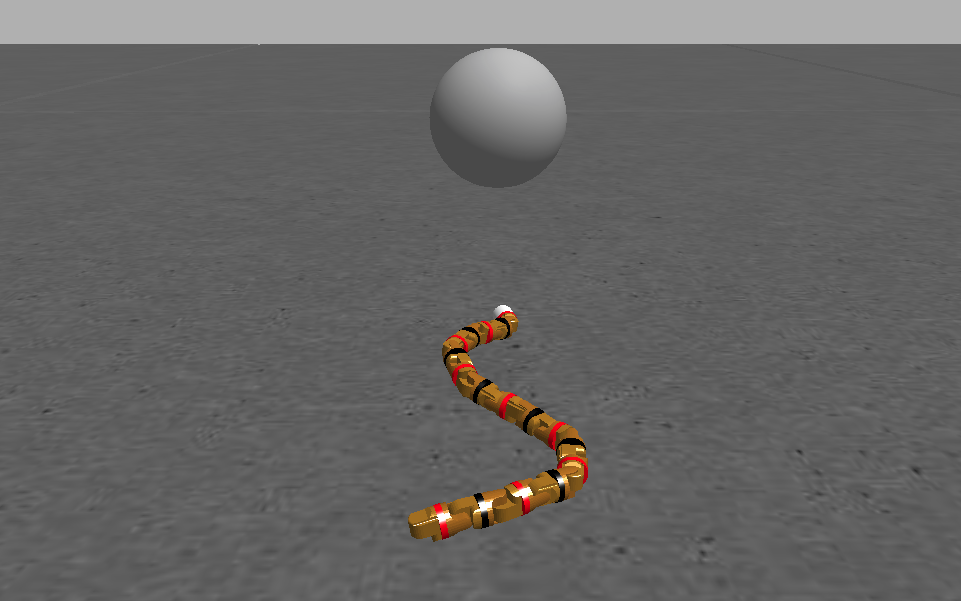
\includegraphics[width=\textwidth]{figures/startingPosition.png}
  \caption{View of the simulation in the starting/reset configuration }
  \label{fig:startingPosRobo}
\end{figure}



\section{Transmitting DVS}
Simulating real DVS data is difficult as the time resolution of DVSs is much higher than the simulation step size. For the experiments a Gazebo plugin developed by Kaiser and Colleagues was used simulating a DVS data stream\cite{kaiser2016towards}. The plugin uses the information provided by a virtual camera mounted in the snakes head to calculate the difference in brightness for each pixel compared to the buffered value of the last timestep. For each pixel exceeding the threshold of $10$ percent a DVS event is created. 
As result events generated in the simulation all happen at the same time.
In their paper \cite{kaiser2016towards} Kaiser and Colleagues compare the output of the simulated output stream with a real one which is shown in \autoref{fig:realDVS}. It is clearly visible that the simulated output has events only in discrete time intervals and has much less noise then the real data.

\begin{figure}[htpb]
  \centering
  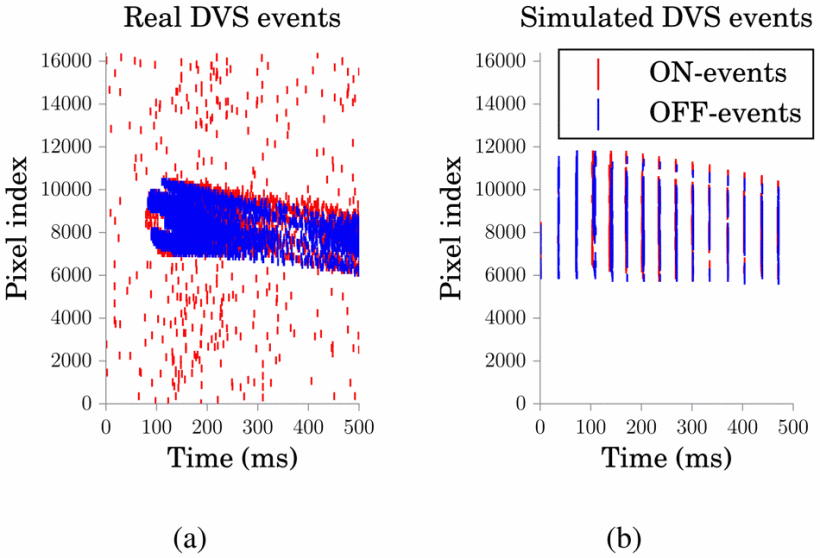
\includegraphics[width=\textwidth]{figures/realDvs.png}
  \caption{Comparison of DVS events generated by a real device (a) and by the simulation (b) \cite{kaiser2016towards}}
  \label{fig:realDVS}
\end{figure}
The simulated sensor has a resolution of $128$ by $128$ pixels. To reduce the complexity of the simulation for the SNN we are not using one input neuron for each pixel but group pixels up to superpixels. Additionally we crob of the bottom $50$ pixel rows as well as the top $20$ pixel rows, as those don't contain as much relevant data as the rest. \autoref{fig:dvsView} shows a rendering of the DVS output at a single simulation timestep and the outlines of the superpixels where in this case two rows of five pixels each were used.

\begin{figure}[htpb]
  \centering
  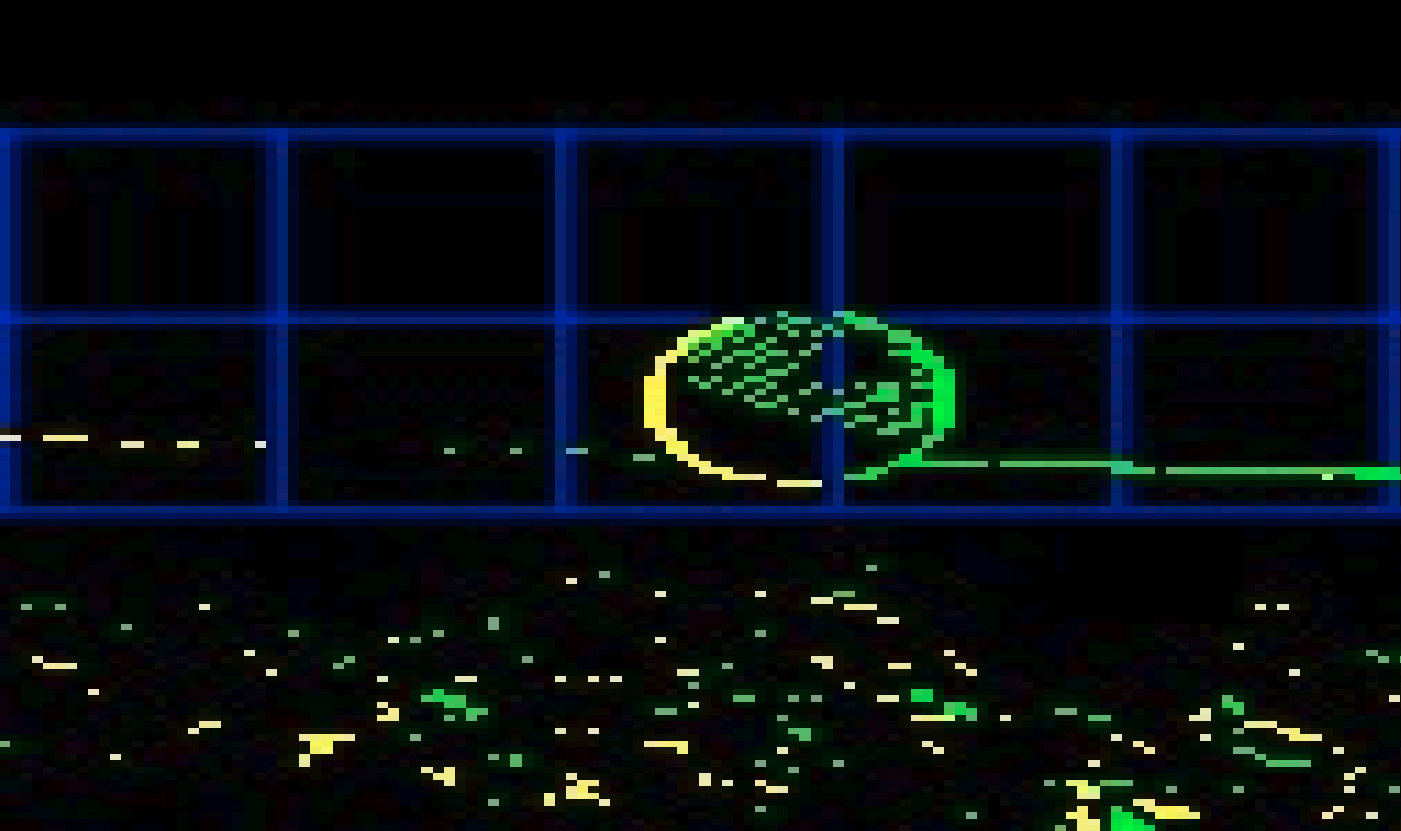
\includegraphics[width=\textwidth]{figures/DvsView.png}
  \caption{Snapshot of the output from the simulated DVS device. The blue lines show the boarder of the superpixels}
  \label{fig:dvsView}
\end{figure}

As the events occur all at the same time but represent the accumulated change over the past timestep, the events are spread out over one timestep. This is done by sending spikes to the network at a certain frequency, proportional to the number of spikes, $N_{events}$, the superpixel received. The frequency $f$ is then calculated by the following function:
\begin{equation}
  f = N_{events} * 50
\end{equation}
The factor at the end results from the simulation timestep lasting one fiftieth of a second thus the frequency $f$, measured in $Hz$, must be $50$ times that high.  Each superpixel has a corresponding Poisson neuron as input for the neural network, which is set to spike at the calculated frequency for the next timestep.
\newline
The input neurons are represented as array with its IDs counting the superpixel from left to right and bottom to top.

\section{Encoding of Joint Angles}\label{sec:EnOfJoint}
For some experiments the angle of some joints of the robot are used as an additional input for the neural network. Each joint angle is represented by two poisson neurons, one spiking proportional to the positive angle, one proportional to the negative angle. The angle $\beta$ is measured from the orientational axe of the module the joint is mounted on (module 1), which is shown in \autoref{fig:robAngle}

\begin{figure}[htpb]
  \centering
  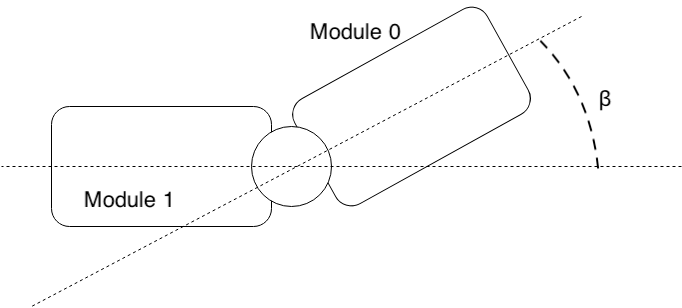
\includegraphics[width=\textwidth]{figures/roboAngle.png}
  \caption[Sketch of joint angle]{This sketch shows how the angle for a joint is measured. The angle $\beta$ of the joint between the two modules would be in this case around $-30$ degree}
  \label{fig:robAngle}
\end{figure}


With this setup only one neuron is active at a time and it’s spike frequency is given by the following equation:
\begin{equation}
  f_R = max(0., a * c)
\end{equation}
for the neuron signaling a positive angle and 
\begin{equation}
  f_L = max(0., - a * c)
\end{equation}
for the neuron signaling a negative angle. In the functions $a$ is the angle of the joint in degree and $c$ is a constant coefficient. This can be interpreted as the activity of neurons controlling the antagonist or respectively the agonist of a joint.

\section{Output Decoding}\label{sec:OutputDecoding}
The output for the used network is as well represented by two neurons, one for signaling the intention to go right, one for going left. To access the total number of spikes occurred on the outputs, each is connected to a spike recorder which keeps track of the spike history.
After each simulation step the number of spikes at the output is retrieved from its spike recorder and the spike recorder gets reset. From the difference in spike events the general direction is derived. This is then scaled by the mean number of spike events occurred on the nodes,which is shown in the following functions:
\begin{equation}
  N_d = N_r - N_l \\
\end{equation}
\begin{equation}
  D = N_d / (0.5 * (N_r + N_l)) \text{, with $D=[-2;2]$} 
\end{equation}
\begin{equation}
  D_{norm} = 0.5 * D = N_d/(N_r+N_l) 
\end{equation}
where $N_r$ and $N_l$ are the total number of spikes for the right/left neuron, $D_{norm}$ can be seen as the direction scaled by certainty, as its absolute value gets bigger the more exclusive the spikes occur on one neuron. By this interpretation of $D_{norm}$ representing the intention of changing the current direction $D_{t-1}$, the resulting direction $D_t$ is calculated by 
\label{eg:OutputCalc}
\begin{equation}
  D_t = min(1,max(-1,( D_{t-1} + D_{norm} * c_{imp})))
\end{equation}
Where $c_{imp}$ is a constant coefficient scaling how aggressive the direction can be changed. $D_t$ should always be in the range of $-1$ to $1$ as the robot has a finite steering range on which $D_t$ then gets projected.

\section{Reward Assignment}\label{sec:rewardAss}
For the network to learn a reward has to be given depending on its performance. There for finding a suitable reward function is crucial for successful training of the network.
In this thesis the reward is defined through the angle to the target as shown in \autoref{eq:reward}.
\begin{equation}\label{eq:reward}
r_{left/right} = -/+ a * c_{rew}
\end{equation}
As can be seen the reward for the left and right neuron scale linear by the coefficient $c_{rew}$ with opposing signs. Is the angle to the target $a$ negative the connection to the left neuron get a positive reward and vice versa. This way connections consistently taking part in firing the left neuron while the target is left and are not taking part firing it while the target is right will increase in weight.
To remove additional steps and as it scales better to SNNs with hidden layers, the reward is assigned directly to the synapses rather than exciting a neuron which triggers the release of dopamine to the synapses.
\autoref{eq:reward} assigns only reward to the connections before the output layer. And the reward is assigned counteracting the overall error, the absolute angle to the target. For neurons in hidden layers this isn’t trivial anymore but can be solved with a method similar to the backpropagation algorithm introduced in \autoref{sec:backprop}
In this case the reward is propagated backwards where the reward for a neuron should be proportional to the reward the neurons it connects to receive scaled by the weighted of that connections. This process is described in the paper of Bing, Jiang \cite{bing2019end} which was released earlier this year. The reward for the j-th neuron in the i-th layer counted bottom up is given by
\begin{equation}\label{eq:rewardProp}
r_{i,j} = 
\frac{ \sum_{k=1}^{Y_i-1}( r_{i-1,k} * w_{i,j,k}) }
	{ max( |w_{i,j,1}|, |w_{i,j,Y_{i-1}-1}|, |w_{i,j,Y_{i-1}}| ) * Y_{i-1}  } 
\end{equation}
where $Y_{i-1}/Y_{i}$ is the number of neurons in the $(i-1)-th$ respectively in the $i-th$ layer, $r_{i-1,k}$ the reward of the $k-th$ neuron in the$(i-1)-th$ layer with the weight $w_{i,j,k}$ of the synapse connecting to it. In the divisor the maximum absolute weight of the outgoing connections, from the neuron the reward is calculated for, is multiplied by the number of neurons it connects to.

As an example a multilayered SNN with one hidden layer is assumed where the hidden layer is fully connected with the output layer which consists of two neurons. For each neuron in the hidden layer the reward has to be calculated using \autoref{eq:rewardProp}. As shown in \autoref{fig:MSNNfull} this means that a single neuron in the hidden layer only has two outgoing synapses, one for each output.

\begin{figure}[htpb]
  \centering
  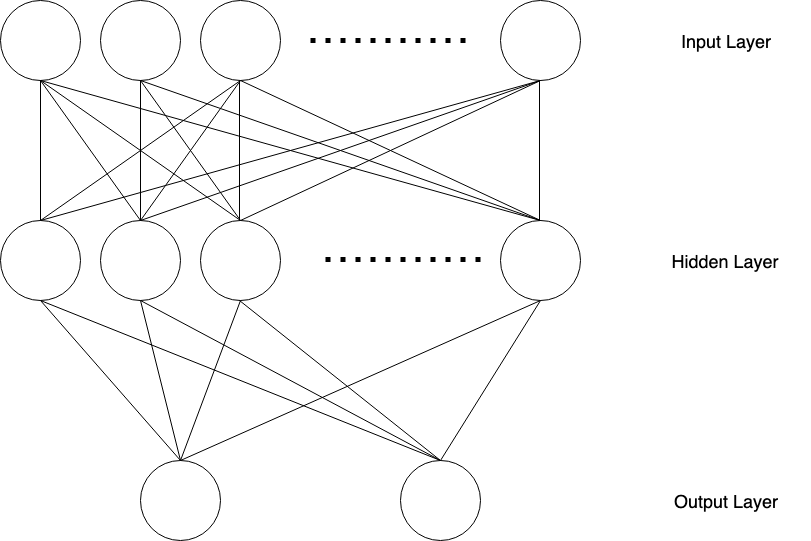
\includegraphics[width=\textwidth]{figures/MSNNfu.png}
  \caption{Schematic of a multilayerd SNN with two output neurons}
  \label{fig:MSNNfull}
\end{figure}
With $r_{l/r}$ as the reward for the left/right neuron and $w_{l/r}$ the connection for this neuron to the left/right output \autoref{eq:rewardProp} simplifies to
\begin{equation}
r_h = \frac{ r_l * w_l + r_r * w_r} {max(|w_l|,|w_r|)*2}
\end{equation}
As the reward defined in \autoref{eq:reward} has the same value with opposing signing the last equation resolves to
\begin{equation}\label{eq:rewardPSimp}
r_h = \frac{ -r_r * w_l + r_r * w_r} {max(|w_l|,|w_r|)*2}
\end{equation}
\begin{equation*}
  r_h = \frac{ r_r *(w_r-w_l) } {max(|w_l|,|w_r|)*2}
\end{equation*}
In this manner the reward for each neuron can be calculated.
